\documentclass[12pt, psamsfonts]{amsart}

%-------Packages---------
\usepackage{amssymb,amsfonts}
\usepackage{fullpage}
\usepackage{todonotes}
\usepackage{physics}
\usepackage[all,arc]{xy}
\usepackage{enumerate}
\usepackage{mathrsfs}
\usepackage{theoremref}
\usepackage{graphicx}
\usepackage[bookmarks]{hyperref}

%--------Theorem Environments--------
%theoremstyle{plain} --- default
\newtheorem{thm}{Theorem}[section]
\newtheorem{cor}[thm]{Corollary}
\newtheorem{prop}[thm]{Proposition}
\newtheorem{lem}[thm]{Lemma}
\newtheorem{conj}[thm]{Conjecture}
\newtheorem{quest}[thm]{Question}

\theoremstyle{definition}
\newtheorem{defn}[thm]{Definition}
\newtheorem{defns}[thm]{Definitions}
\newtheorem{con}[thm]{Construction}
\newtheorem{exmp}[thm]{Example}
\newtheorem{exmps}[thm]{Examples}
\newtheorem{notn}[thm]{Notation}
\newtheorem{notns}[thm]{Notations}
\newtheorem{addm}[thm]{Addendum}
\newtheorem*{exer}{Exercise}

\theoremstyle{remark}
\newtheorem{rem}[thm]{Remark}
\newtheorem{rems}[thm]{Remarks}
\newtheorem{warn}[thm]{Warning}
\newtheorem{sch}[thm]{Scholium}

\DeclareMathOperator{\Hom}{Hom}
\DeclareMathOperator{\Id}{Id}

\makeatletter
\let\c@equation\c@thm
\makeatother
\numberwithin{equation}{section}

\bibliographystyle{plain}

\begin{document}

\title{Math 611 Homework (Due 9/25)}
\author{Hidenori Shinohara}
\maketitle

\begin{exer}{(Problem 4, Chapter 1.3)}
  Construct a simply-connected covering space of the space $X \subset \mathbb{R}^3$ that is the union of a sphere and a diameter.
  Do the same when $X$ is the union of a sphere and a circle intersecting it in two points.
\end{exer}

\begin{proof}
  \begin{figure}
    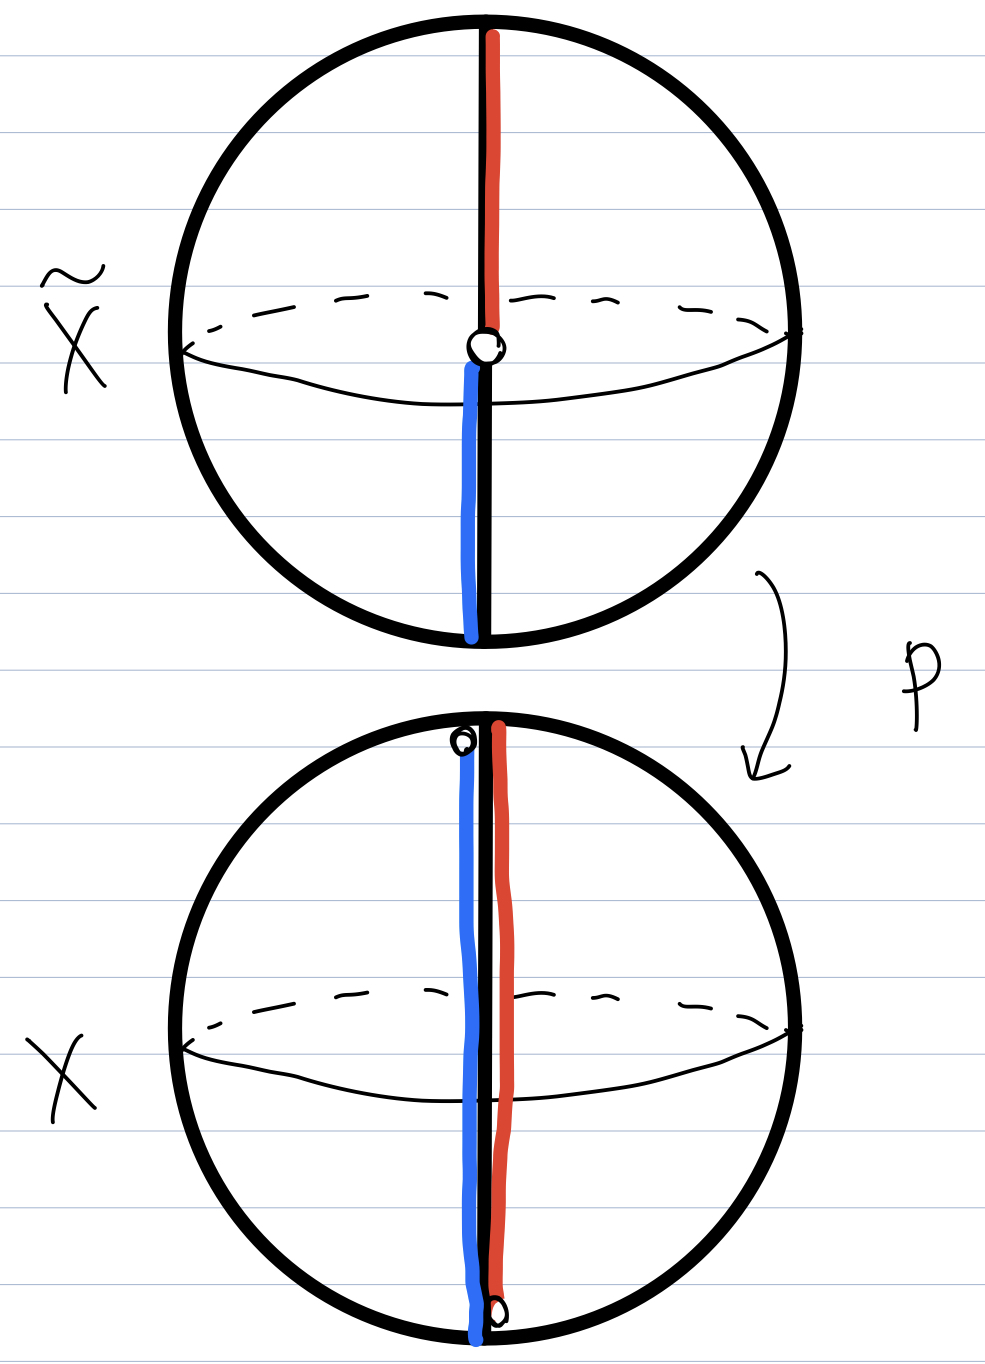
\includegraphics[width=.5\linewidth]{problem4-1.jpeg}
    \caption{Problem 4 (Part 1)}
    \label{fig:prob4_1}
  \end{figure}
  We claim that the space described in Figure \ref{fig:prob4_1} is a covering space of $X$.
  \begin{itemize}
    \item
      The shape is an infinitely long chain of spheres and lines.
      The chain goes infinitely both ways (up and down).
      This space is clearly simply connected.
    \item
      We will map each sphere to the sphere of $X$.
      Each line will be mapped to the diameter up side down.
      Figure \ref{fig:prob4_1} shows how each part gets mapped.
    \item
      We claim that such a mapping is a covering map and thus this infinite chain is indeed a covering space.
      Let $x \in X$.
      \begin{itemize}
        \item
          If $x$ is on the diameter and disjoint from the sphere, a neighborhood that is disjoint from the sphere is evenly covered.
        \item
          If $x$ is on the sphere and disjoint from the diameter, a neighborhood that is disjoint from the diameter is evenly covered.
        \item
          If $x$ is the north pole, a neighborhood that does not contain the south pole is evenly covered.
        \item
          If $x$ is the south pole, a neighborhood that does not contain the north pole is evenly covered.
      \end{itemize}
  \end{itemize}
  Therefore, the space described in Figure \ref{fig:prob4_1} is a covering space of $X$.
  \begin{figure}
    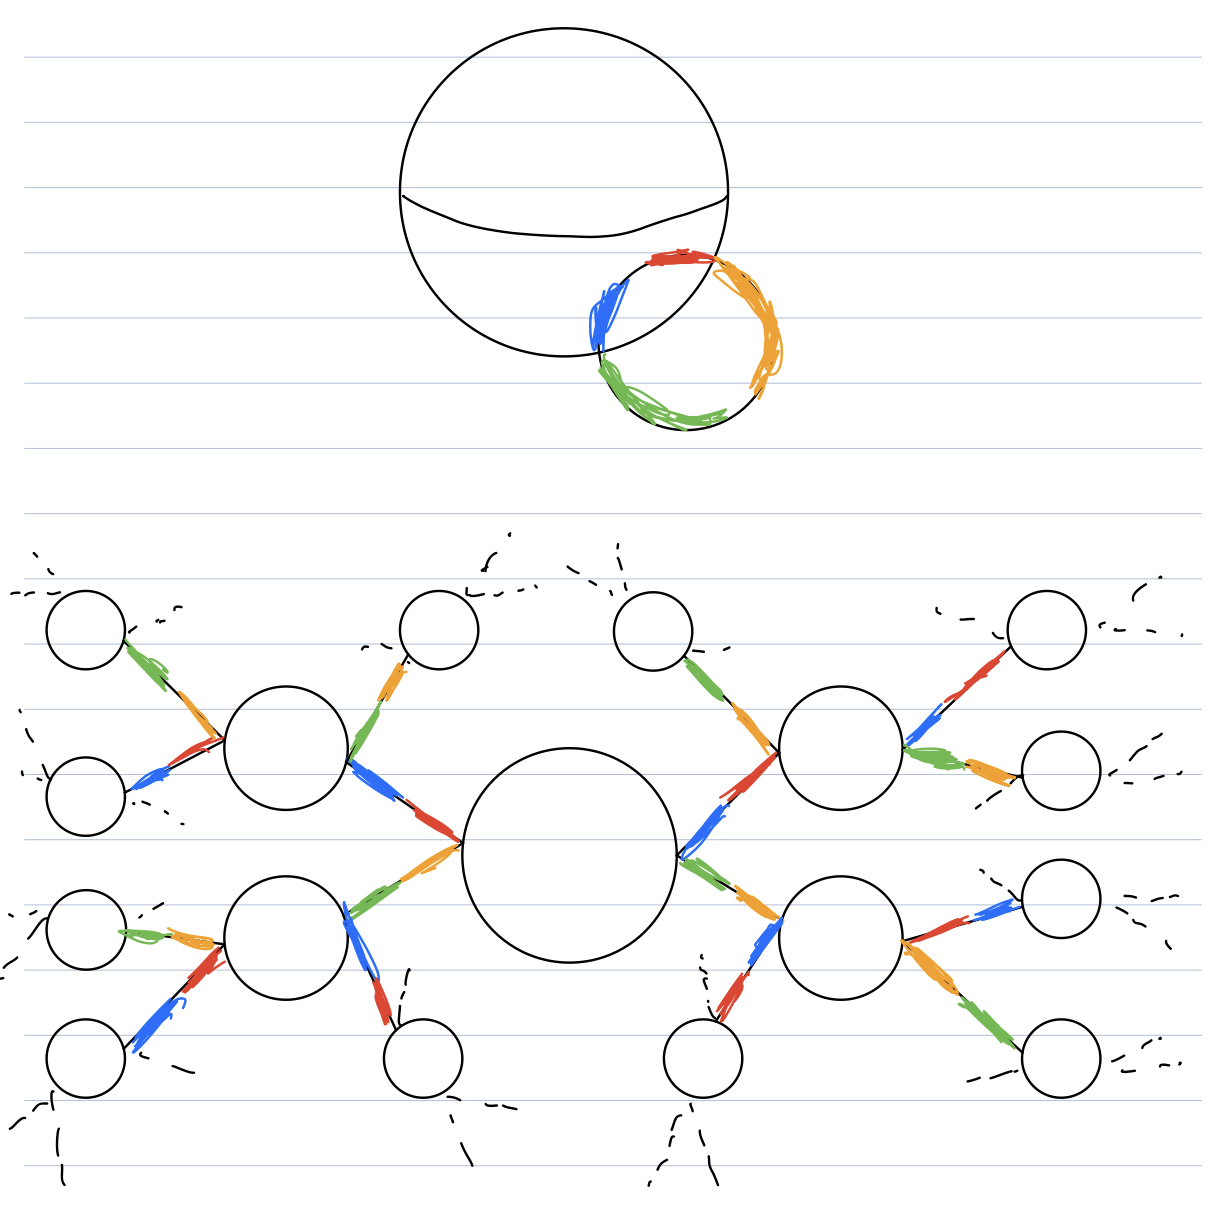
\includegraphics[width=.5\linewidth]{problem4-2.jpeg}
    \caption{Problem 4 (Part 2)}
    \label{fig:prob4_2}
  \end{figure}

  Figure \ref{fig:prob4_2} has an example of a simply-connected covering space of $X$.
  This space can be constructed by first having a sphere in the middle.
  4 edges should be attache at two points of the sphere.
  And each edge should be connected to a different sphere.
  We continue attaching them such that each sphere has exactly two points each of which has two edges.
  The edges should be mapped to the circle as described in \ref{fig:prob4_2} by 4 different colors.
  It is clear that each point has an evenly covered neighborhood.
\end{proof}

\begin{exer}{(Problem 5, Chapter 1.3)}
  Let $X$ be the subspace of $\mathbb{R}^2$ consisting of the four sides of the square $[0, 1] \times [0, 1]$ together with the segments of the vertical lines $x = 1/2, 1/3, 1/4, \cdots$ inside the square.
  Show that for every covering space $X \rightarrow X$ there is some neighborhood of the left edge of $X$ that lifts homeomorphically to $\tilde{X}$.
  Deduce that $X$ has no simply-connected covering space.
\end{exer}

\begin{proof}
  For each $y \in [0, 1]$, the point $(0, y)$ has a neighborhood $U_y$ that is evenly covered.
  Then there exists an open rectangle $R_y \subset \mathbb{R}^2$ such that $y \in R_y \cap Y \subset U_y$.
  Since any open subset of an evenly covered set is evenly covered, such $R_y \cap Y$ is evenly covered.
  Let $V_y$ denote $R_y \cap Y$ for each $y$.
  $\{ V_y  \mid y \in [0, 1] \}$ is an open cover of the segment $\{ 0 \} \times [0, 1]$.
  Since the segment is compact, there exists a finite subcover, $V_{y_1}, \cdots, V_{y_k}$.

  Since we found a finite cover where each of them is rectangular shaped, there exists an $N \in \mathbb{N}$ such that $\forall n \geq N, \{ 1/n \} \times [0, 1] \subset \bigcup_{i=1}^{n} V_{y_i}$.
  Since each $V_{y_1}, \cdots, V_{y_k}$ is a subset of an open rectangle, there must exist a partition $0 = t_0 < t_1 < \cdots < t_m = 1$ such that for all $i$, $[0, 1/N] \times [t_i, t_{i + 1}]$ is contained in an evenly covered open subset.
  We will inductively show that $[0, 1/N] \times [0, t_i]$ is contained in an evenly covered open subset.
\end{proof}

\begin{exer}{(Problem 7, Chapter 1.3)}
  Let $Y$ be the quasi-circle in the figure in the textbook.
  Collapsing the segment of $Y$ in the $y$-axis to a point gives a quotient map $f: Y \rightarrow S^1$.
  Show that $f$ does not lift to the covering space $\mathbb{R} \rightarrow S^1$, even though $\pi_1(Y) = 0$.
  Thus local path-connectedness of $Y$ is a necessary hypothesis in the lifting criterion.
\end{exer}

\begin{proof}
  \todo[inline]{
    The lifting criterion is Proposition 1.33.
    The only property that $Y$ is missing is the local path connectedness.
    I need to understand the proof because I essentially have to find where the proof goes wrong if local path connectedness is missing.
    I think what happens is that if $\tilde{f}$ existed, it would have to be unique.
    Thus we could look into the one function that could possibly be $\tilde{f}$.
    Since the local connectedness is used to prove continuity of $\tilde{f}$ and $Y$ is not locally connected around the $[-1, 1]$ segment, I would guess that that one function is not continuous at a point on the $[-1, 1]$ segment.
    See Figure \ref{fig:problem7}.
  }
  \begin{figure}
    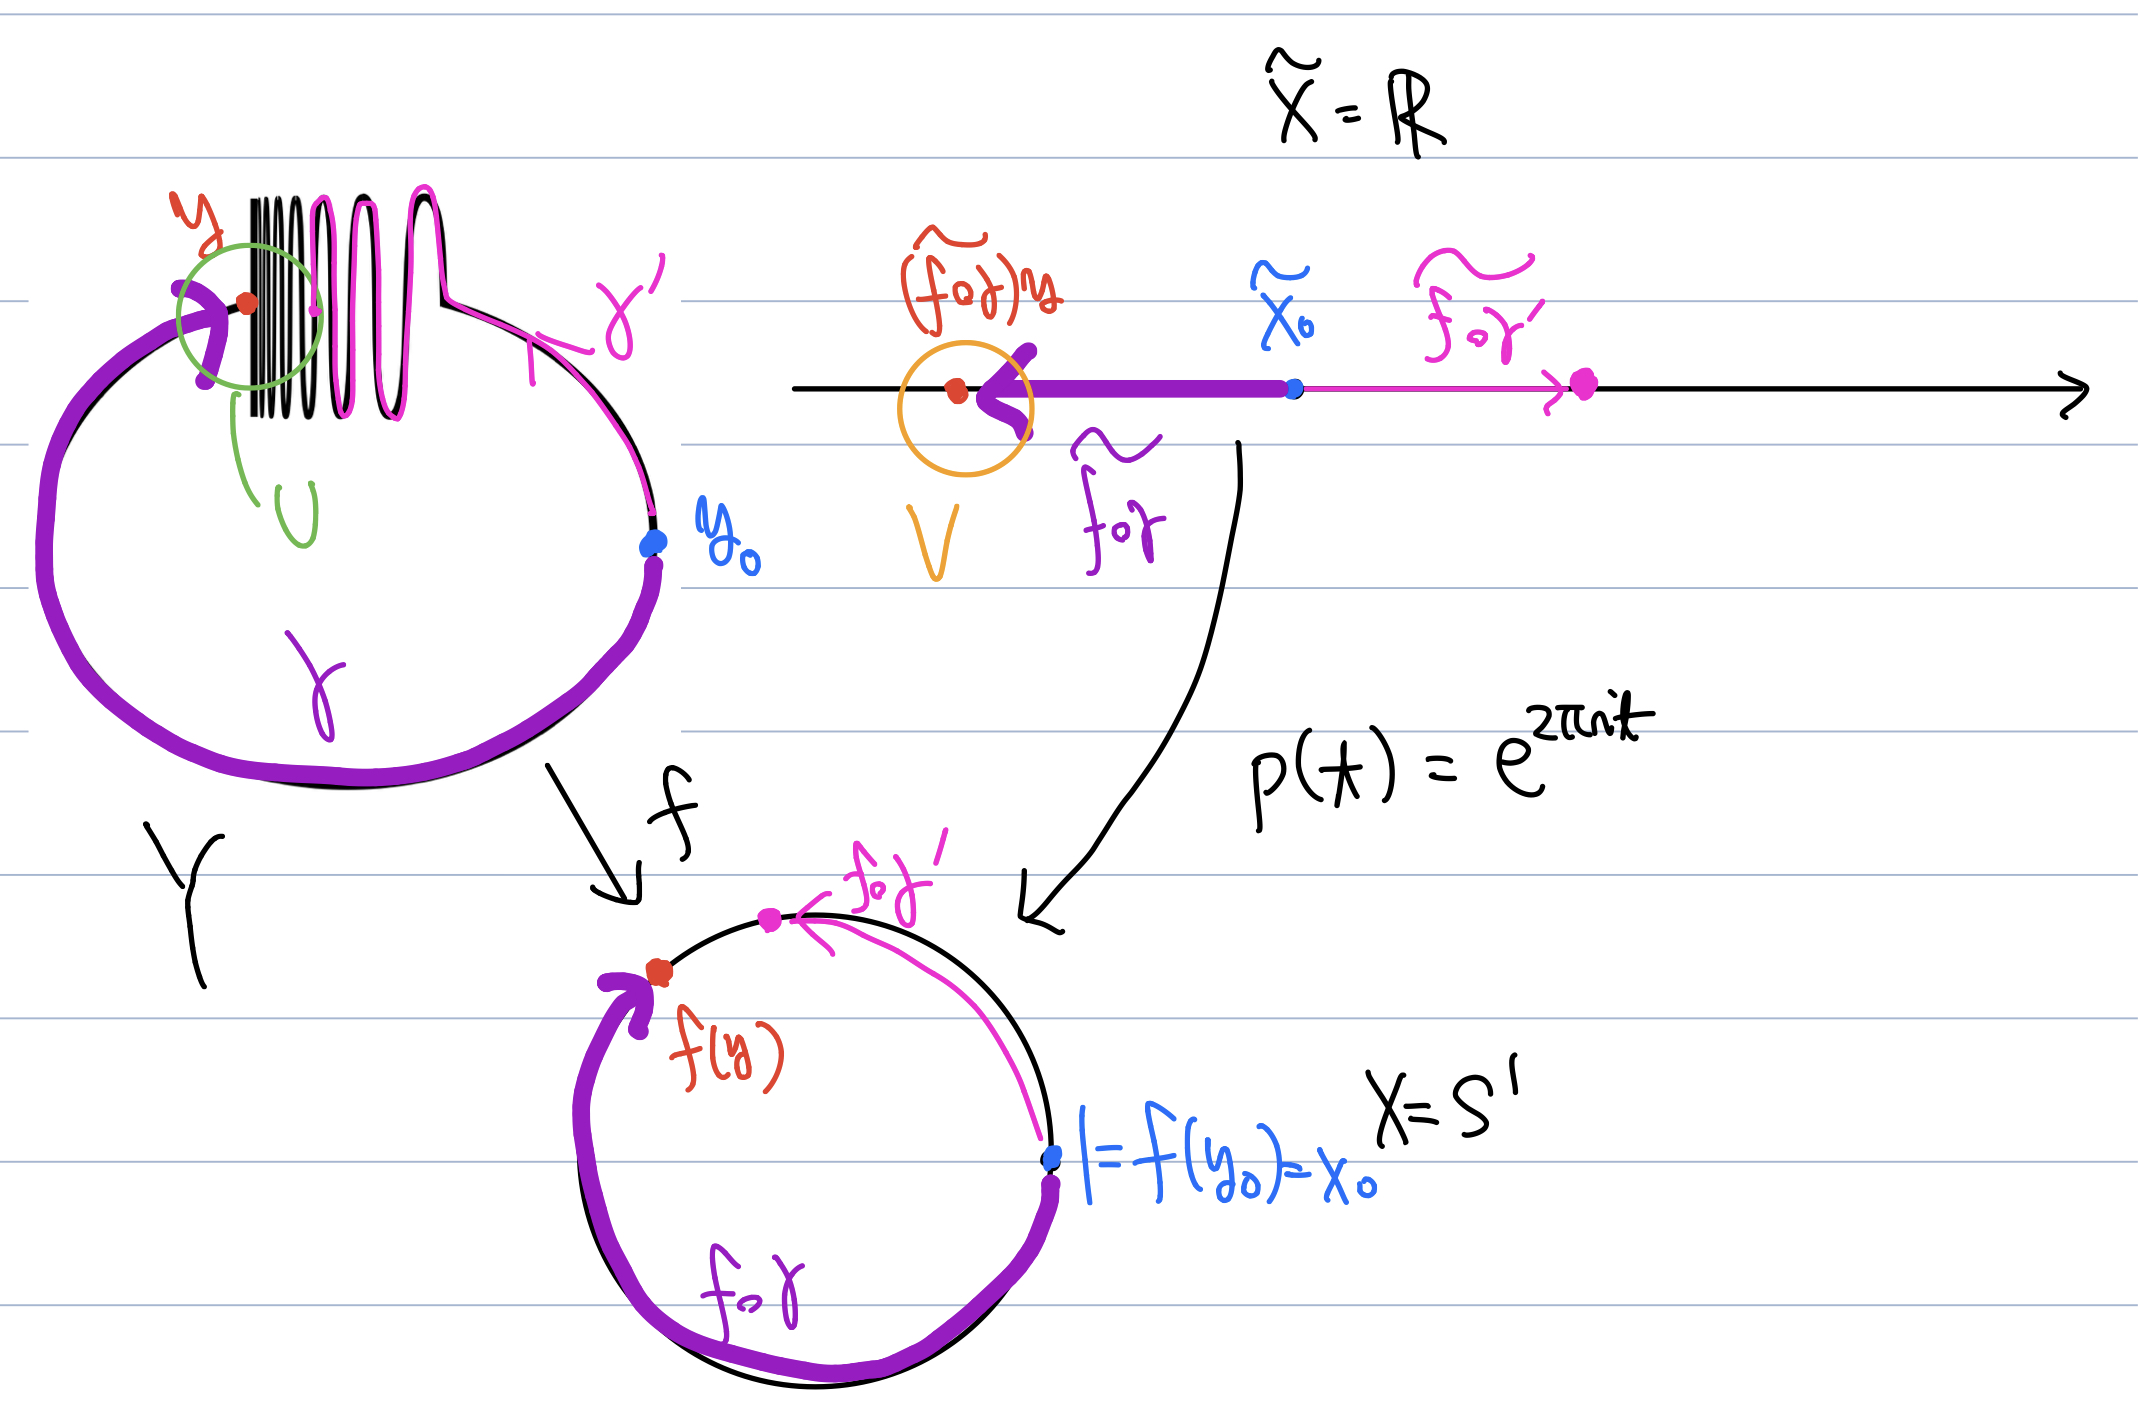
\includegraphics[width=.5\linewidth]{problem7.jpeg}
    \caption{Delete this!}
    \label{fig:problem7}
  \end{figure}
\end{proof}

\begin{exer}{(Problem 8, Chapter 1.3)}
  Let $\tilde{X}$ and $\tilde{Y}$ be simply-connected covering spaces of the path-connected, locally path-connected spaces $X$ and $Y$.
  Show that if $X \simeq Y$ then $\tilde{X} \simeq \tilde{Y}$.
\end{exer}

\begin{proof}
  \todo[inline]{
    By Proposition 1.33, we can lift the two compositions as in Figure \ref{fig:problem8}.
    This works because $\pi_1(\tilde{X}) = \pi_1(\tilde{Y}) = 0$.
    I'm not sure how Exercise 11 (Chapter 0) helps, but I solved the first part of it.
    Let $F$ be a homotopy between $f \circ g$ and $\Id$, and let $H$ be a homotopy between $h \circ f$ and $\Id$.
    Let $G$ be defined such that $G_t = h \circ F_{2t} \circ f$ for $t \in [0, 1/2]$, and $G_t = H_{2t - 1}$ for $t \in [1/2, 1]$.
    I should try the second part to see if that helps me.
  }
  \begin{figure}
    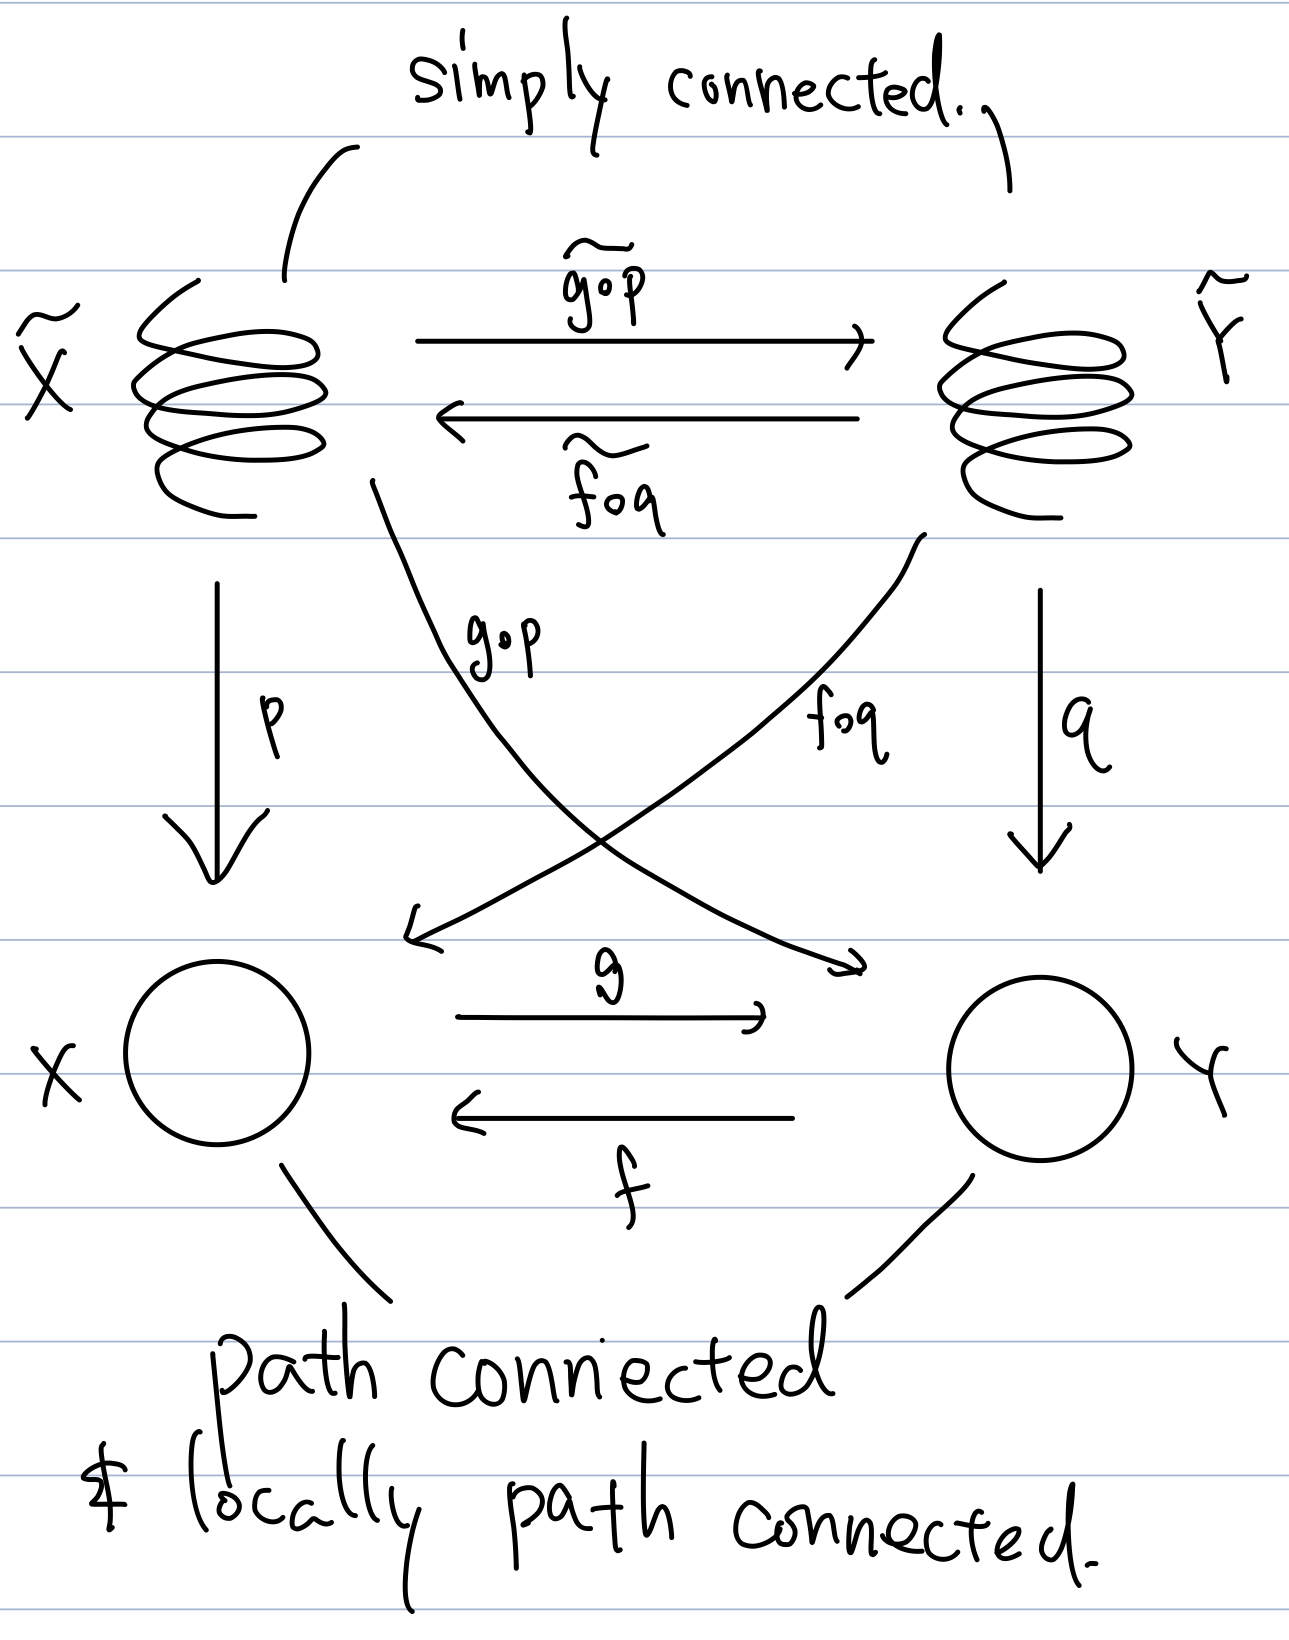
\includegraphics[width=.5\linewidth]{problem8.jpeg}
    \caption{delete this!}
    \label{fig:problem8}
  \end{figure}
\end{proof}


\end{document}


